\documentclass[spanish]{article}
\usepackage{titlesec}



%\usepackage[spanish]{babel} ¡Esto estaba interfiriendo con las flechitas de los \tikspicture

\renewcommand{\contentsname}{Índice}

\usepackage[left=4cm, right=4cm]{geometry}
\usepackage{palatino}%Font
\usepackage{graphicx}
\usepackage{wrapfig}
\usepackage{marvosym}%Smileys
\usepackage{float}
\usepackage{subcaption}
\usepackage{enumitem}
\usepackage{parskip}
\usepackage{amsthm}
\usepackage{amssymb}
\usepackage{amsmath}
\usepackage{stmaryrd}
\usepackage{pst-solides3d}
\usepackage{tikz}
\usepackage{tikz-cd}
\usetikzlibrary{shapes.geometric}
\usetikzlibrary{%
	matrix,%
	calc,%
	arrows,%
	shapes,
	decorations,
	decorations.markings
}
\usetikzlibrary{arrows, arrows.meta}
\usepackage[bookmarks,bookmarksopen,bookmarksdepth=3]{hyperref}
\hypersetup{
	colorlinks=true,
	urlcolor=blue,
	linkcolor=magenta,
	citecolor=blue,
	filecolor=blue,
	urlbordercolor=white,
	linkbordercolor=white,
	citebordercolor=white,
	filebordercolor=white
}

\theoremstyle{definition}
\renewcommand{\proofname}{Demostración}

\newtheorem*{defn}{Definición}
\newtheorem*{lema}{Lema}
\newtheorem*{obs}{Observación}
\newtheorem*{teo}{Teorema}
\newtheorem*{prop}{Proposición}
\newtheorem*{coro}{Corolario}
\newtheorem*{af}{Afirmación}
\newtheorem*{ejer}{Ejercicio}
\newtheorem*{ejem}{Ejemplo}
\newtheorem*{pregunta}{Pregunta}

\newcommand{\R}{\mathbb{R}}
\newcommand{\Z}{\mathbb{Z}}
\newcommand{\N}{\mathbb{N}}
\newcommand{\C}{\mathbb{C}}
\newcommand{\Q}{\mathbb{Q}}
\newcommand{\Hy}{\mathbb{H}}
\newcommand{\A}{\mathbb{A}}
\newcommand{\D}{\mathbb{D}}
\newcommand{\M}{\mathbb{M}}
\DeclareMathOperator{\Id}{Id}
\DeclareMathOperator{\img}{img}
\DeclareMathOperator{\rel}{rel}
\DeclareMathOperator{\Mod}{Mod}
\DeclareMathOperator{\Hom}{Hom}
\DeclareMathOperator{\Homeo}{Homeo}
\DeclareMathOperator{\Isom}{Isom}
\DeclareMathOperator{\Deck}{Deck}
\DeclareMathOperator{\Diff}{Diff}
\DeclareMathOperator{\SL}{SL}
\DeclareMathOperator{\PSL}{PSL}
\DeclareMathOperator{\SMod}{\mathcal{S}Mod}
\DeclareMathOperator{\LMod}{\mathcal{L}Mod}
\DeclareMathOperator{\SHomeo}{\mathcal{S}Homeo}
\DeclareMathOperator{\LHomeo}{\mathcal{L}Homeo}

\usepackage[backend=bibtex]{biblatex}
\addbibresource{bir.bib}

\title{Teoría de Birman-Hilden}

\begin{document}
	\maketitle
	\phantomsection
	\addcontentsline{toc}{part}{\contentsname}
	\tableofcontents
	

\section{Cubrientes}
En la demostración del grupo fundamental del círculo ya habíamos usado la idea de espacio cubriente. Aquí está la definición general:
\begin{defn}
	Un \textbf{espacio cubriente} de $X$ es un espacio $E$ junto con una función \[p:E\to X\] tal que cada punto $x\in X$ tiene una vecindad abierta $U\subseteq X$ tal que $p^{-1}(U)$ es una unión disjunta de abiertos de $E$ de manera que cada uno se proyecta homeomorfamente a $U$ vía $p$.
\end{defn}
\begin{wrapfigure}[13]{l}{0.33\textwidth}
	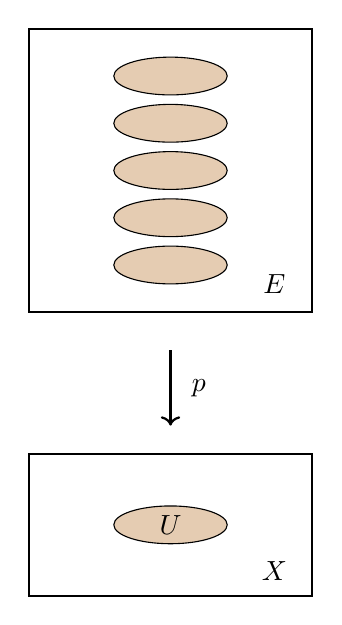
\begin{tikzpicture}[scale=1.2]
		% Rectangle representing X
		\draw[thick] (0,0) rectangle (3,1.5);
		\node at (1.5,0.75) {X};
		
		% Pancake U inside X
		\draw[fill=brown!40] (1.5,0.75) ellipse (0.6 and 0.2);
		\node at (1.5,0.75) {$U$};
		\node at (2.6,0.26) {$X$};
		
		% Rectangle representing  E
		\draw[thick] (0,3) rectangle (3,6);
		\node at (2.6,3.3) {$ E$};
		
		% Stacked pancakes above U
		\def\numpans{5}
		\def\pancakeHeight{0.2}
		\def\pancakeSpacing{0.3}
		\def\tildeXtop{6.2}
		
		\foreach \i in {1,...,\numpans} {
			\pgfmathsetmacro\yshift{\tildeXtop - \i*(\pancakeHeight + \pancakeSpacing)}
			\draw[fill=brown!40] (1.5,-0.2+\yshift) ellipse (0.6 and \pancakeHeight);
		}
		% Arrow from  E to X
		\draw[->, thick] (1.5,2.6) -- (1.5,1.8);
		\node at (1.8,2.2) {$p$};
	\end{tikzpicture}
	\vspace{-2.6cm}
\end{wrapfigure}
Introducimos otros términos:
\begin{itemize}
	\item A la función $p$ le llamamos \textbf{proyección cubriente}.
	\item A $U$ se le llama \textbf{vecindad regular}.
	\item A los abiertos de $p^{-1}(U)$ que se proyectan homeomorfamente a $U$ se les llama \textbf{hojas} de $E$ sobre $U$.
	\item El conjunto $p^{-1}(x)$ se llama la \textbf{fibra} de $x$ bajo $p$.
\end{itemize}
\begin{obs}\leavevmode
	\begin{itemize}
		\item Si $U$ es conexo entonces las hojas de $U$ son las componentes conexas de $p^{-1}$.
		\item El número de hojas sobre $U$ es igual a la cardinalidad de $p^{-1}(x)$.
		\item Este número es \textit{localmente constante}, es decir, es igual para cualquier punto:
	\end{itemize}
\end{obs}\vspace{1cm}

\begin{ejem}\leavevmode
	\begin{enumerate}
		\item La identidad $Id:X\to X$.
		\item La proyección natural de la unión disjunta de copias de un espacio, es decir $p:\bigsqcup_{\alpha\in I}X\to X$.
		\item Para cualesquiera dos cubrientes $p: E\to X$ y $q:\tilde{E}\to X$, la proyección desde la unión disjunta $r: E\sqcup\tilde{E}\to X$ definida de la manera natural, también es un cubriente. Esto para decir que nos interesan los cubrientes de espacios conexos cuyos cubrientes sean conexos.
		\item $p:\R\to S^1$ como en la prueba del grupo fundamental del círculo.
		\item Para $n\in\N$, la función	$p:S^1\to S^1$ dada por $p(z)=z^n$
	\end{enumerate}
\end{ejem}
\section{Acciones de un grupo en un espacio topológico}
\begin{defn}
	Decimos que un grupo $G$ \textbf{actúa} en $X$ si hay un homomorfismo de grupos
	\begin{align*}
		\varphi:G\to\Homeo(X)\\
		g\mapsto\varphi(g):X\to &X\\
		x\mapsto&\varphi(g)(x)
	\end{align*}
	de forma que
	\begin{itemize}
		\item  $\varphi(g_1g_2)=\varphi(g_1)\varphi(g_2)$
		\item $(g_1g_2)x=g_1(g_2(x))$
		\item $\varphi(1_G)=Id_X$
	\end{itemize}
	Y se denota $G\curvearrowright X$. Una acción es \textbf{libre} si $g(y)=y$ para cualesquiera $g\in G$ y $y\in Y$, implica que $g=1_G$; y una acción es \textbf{transitiva} si para cualesquiera $y,y'\in Y$ existe un elemento $g\in G$ tal que $g\cdot y=y'$.
	
	Denotaremos el \textbf{espacio de órbitas} por $X/G:=\{G\cdot x:x\in C\}$.
\end{defn}
\begin{obs}
	No cualquier grupo finito induce una acción libre en un espacio dado. Por ejemplo, $\Z/2\Z\approx\{Id,-Id\}$ actuando en todo $\R^2$ fija al origen.
\end{obs}
\section{Levantamientos}
	Comenzamos recordando el criterio de levantamiento de funciones:
Consideremos un cubriente $p: E\to X$ y una función cualquiera $f:Y\to X$. Queremos que este diagrama conmute:
\[\begin{tikzcd}[column sep=1cm,row sep=1cm]
	& E\arrow[d,"p"]\\
	Y\arrow[ur,dashed,"\tilde{f}"]\arrow[r,swap,"f"]&X
\end{tikzcd}\]
\begin{prop}[Unicidad del levantamiento]
	Sean $p: E\to X$ un cubriente y $f:Y\to X$ una función. Si dos levantamientos $\tilde{f}_1,\tilde{f}_2:Y\to E$ de $f$ coinciden en un punto y $Y$ es conexo, entonces $\tilde{f}_1=\tilde{f}_2$.
	\[\begin{tikzcd}
		& E\arrow[d,"p"]\\
		Y\arrow[ru,"\tilde{f}_1"]\arrow[ru,swap,"\tilde{f}_2"]\arrow[r,swap,"f"]&X
	\end{tikzcd}\]
\end{prop}
\begin{teo}[Propiedad del levantamiento de homotopía para cubrientes]\label{teo-lhc}
	Dado un cubriente $p: E\to X$ y una homotopía $h_t:Y\to X$ y un levantamiento $\tilde{f}_0:Y\to  E$ de $f_0$, entonces existe una única homotopía $\tilde{f}_t:Y\to  E$ que levanta a cada uno de los $f_t$.
	
	Es decir, que el siguiente diagrama conmuta:
	\[\begin{tikzcd}[column sep=1cm,row sep=1cm]
		Y\times\{0\}\arrow[r,"\tilde{f}_0"]\arrow[rd,"f_0" near end]\arrow[d,hook]& E\arrow[d,"p"]\\
		Y\times I\arrow[r]\arrow[ru,dashed]&X
	\end{tikzcd}\]
\end{teo}
\begin{defn}
	Decimos que un espacio topológico $Y$ es \textbf{localmente arco-conexo} si para todo punto $y\in Y$ y cada vecindad $U$ de $y$, existe $y\in V\subseteq U$ que es arcoconexa.
\end{defn}
\begin{prop}
	Sean $p:( E, E_0)\to (X,x_0)$ un cubriente y una función $f:(Y,y_0)\to (X,x_0)$ con $Y$ espacio arco-conexo y localmente arco-conexo. Entonces existe un levantamiento $\tilde{f}:(Y,y_0)\to( E,x_0)$ si y sólo si $f_*\pi_1(Y,y_0)\subseteq p_*\pi_1( E, E_0)$.
\end{prop}
\begin{defn}
	Un \textbf{levantamiento} de una función $f:Y\to X$ con respecto a un cubriente $p: E\to X$ es una función $\tilde{f}:Y\to E$ tal que $p\tilde{f}=f$. Es decir, que el siguiente diagrama conmute:
	\[\begin{tikzcd}[column sep=1cm,row sep=1cm]
		& E\arrow[d,"p"]\\
		Y\arrow[ur,dashed,"\tilde{f}"]\arrow[r,swap,"f"]&X
	\end{tikzcd}\]
\end{defn}
\section{Transfromaciones de cubierta}
\begin{defn}
	Tomemos un espacio $X$ y algún cubriente $p: E\to X$. Una \textbf{transformación de cubierta} es un isomorfismo de $ E$ en sí mismo, es decir, homeomorfismos que hacen conmutar este diagrama:
	\[\begin{tikzcd}
		 E\arrow[r,"f"]\arrow[d,swap,"p"]& E\arrow[dl,"p"]\\
		X
	\end{tikzcd}\]
	Es decir, $pf=p$
\end{defn}
El conjunto $\Deck( E):=\left\{f: E\to E:f\text{ es transformación de cubierta}\right\}$ tiene estructura de grupo, y le llamaremos \textbf{el grupo de transformaciones de cubierta} o de \textbf{deck}.
%\begin{ejem}
%	El cubriente $f_n:S^1\to S^1$ dado por $z\mapsto z^n$ tiene grupo de transformaciones de cubierta $G(f_n:S^1\to S^1)=\Z/n\Z$. Además, $f_{n*}\pi_1(S^1)=n\Z$. O sea que $G(f_n:S^1\to S^1)\cong\pi_1(S^1)/f_{n*}\pi_1(S^1)$. Y esto no es ninguna casualidad.
%	
%	Además, para el cubriente universal de $S^1$, que es $\exp:\R\to S^1$ también se cumple, ya que el grupo fundamental es trivial, es decir, $G(\exp:\R\to S^1)\cong\Z/\{0\}\cong\Z$.
%\end{ejem}
\begin{prop}
	Si $g,f: E\to E$ son transformaciones de cubierta con $ E$ arco-conexo y tales que existe $x\in E$ con $g(x)=f(x)$, entonces $g=f$.
\end{prop}
\begin{proof}
	Basta pensar que la transformación de cubierta es un levantamiento de la proyección cubriente:
	\[\begin{tikzcd}
		& E\arrow[d,"p"]\\
		 E\arrow[ur,dashed,"f"]\arrow[r,swap,"p"]&X
	\end{tikzcd}\]
	Por el teorema del levantamiento de funciones, $f$ es único una vez que escogemos un punto $y\in f^{-1}(x)$ en la fibra de $x$.
\end{proof}
\begin{defn}
	Decimos que un cubriente $p: E\to X$ es \textbf{regular} si para cualquier $x\in X$ y $ e, e'\in p^{-1}(x)$ existe una transformación de cubierta $f: E\to E$ tal que $f( e)= e'$. Es decir, que el grupo de transformaciones de cubierta actúa transitivamente en las fibras.
\end{defn}
\begin{prop}
	Sea $p:( E, e_0)\to (X,x_0)$ un cubriente con $ E$ y $X$ arco-conexo y localmente arco-conexo. Sea $H=p_*\pi_1( E, e_0)\leq\pi_1(X,x_0)$. Entonces
	\begin{enumerate}[label=\alph*)]
		\item El cubriente es regular si y sólo si $H\trianglelefteq\pi_1(X,x_0)$.
		\item $\Deck( E)\cong N(H)/H$
		donde $N(H)=\left\{g\in\pi_1(X,x_0)|g^{-1}Hg=H)\right\}$
	\end{enumerate}
	En particular, cuando $ E$ es regular, $\Deck( E)\cong\pi_1(X,x_0)/H$. Y si además $ E$ es el cubriente universal, simplemente tenemos que $\Deck( E)\cong\pi_(X,x_0)$.
\end{prop}
\begin{proof}
	La idea es definir un mapeo suprayectivo $\pi_1(X,x_0)\to\Deck(p)$.
\end{proof}
\section{Acción cubriente}
\begin{defn}
	Decimos que $G\curvearrowright Y$ es una \textbf{acción cubriente} si se cumple cualquiera de los dos siguientes condiciones equivalentes:
	\begin{itemize}
		\item Cualquier punto $y\in Y$ tiene una vecindad $U$ tal que $(g_1U\cap g_2U)\neq\emptyset\implies g_1=g_2$
		\item Cualquier punto $y\in Y$ tiene una vecindad $U$ tal que $gU\cap U\neq\emptyset\implies g=1_G$.
	\end{itemize}
	En particular, estas condiciones implican que la acción es libre.
\end{defn}
\begin{prop}
	Dada una acción cubriente $G\curvearrowright Y$,
	\begin{enumerate}[label=\alph*)]
		\item La proyección cociente $p:Y\to Y/G$ dada por $p(y)=Gy$ es un cubriente regular.
		\item Si $Y$ es arco-conexo, $G\approx\Deck(p)$.
		\item Si $Y$ es arco-conexo y localmente arco-conexo, $G\cong\pi_1(Y/G,y_0)/p_*\pi_1(Y,\tilde{y}_0)$
	\end{enumerate}
\end{prop}
\begin{coro}
	Si además $Y$ es simplemente conexo, por b) y por c), $G=G(\tilde{Y})\cong\pi_1(Y/G,y_0)$.
\end{coro}
\begin{prop}
	Dado un cubriente regular $p:E\to X$ con $G=\Deck(p)$. Entonces hay un homeomorfismo $\psi:X\to E/G$ tal que 
	\[\begin{tikzcd}
		E\arrow[d,swap,"p"]\arrow[rd,"\bar{p}"]\\
		X\arrow[r,"\psi"]&E/G
	\end{tikzcd}\]
\end{prop}
\begin{ejem}
	La superficie de género mayor que 3 es cubriente de $S_2$.
\end{ejem}
\begin{teo}
		Si $X$ es una superficie de Riemann simplemente conexa, entonces es conformamente equivalente a una de las siguiente superficies:
		\begin{itemize}
			\item $\C$.
			\item $C\cup \{\infty\}\approx S^2$.
			\item $\Hy^2$.
		\end{itemize}
\end{teo}
\begin{ejem}
	El cubriente universal de las superficies de género mayor o igual que 2 es el plano hiperbólico (recordar a Klein). El cubriente de hecho se puede ver como una isometría local, así que tenemos una métrica hiperbólica en $S_g$.
	
	Las transformaciones de cubierta son isometrías, es decir,
	\[\Deck(p)\leq \Isom^+\Hy^2=\PSL(2,\R)=\SL(2,\R)/A\sim-A\]
	Por aquí acabamos definiendo los grupos Fuschianos como subgrupos discretos de $\PSL(2,\R)$.
\end{ejem}
\begin{ejem}
	La acción de $\Z/3\Z$ en $S_4$ por rotaciones.
\end{ejem}
\begin{ejem}
	El toro identificando puntos antípodas es una botella de Klein. Para verlo, tomamos una mitad del toro y nos fijamos cómo es la identificación en la frontera.
\end{ejem}
\begin{ejer}[\textcolor{magenta}{Tarea}]\leavevmode
	\begin{enumerate}
		\item Consideremos el anterior cubriente $p:T^2\to T^2/\langle\sigma\rangle$. Prueba que todo homeomorfismo de la botella de klein en sí misma admite un levantamiento al toro. (De hecho,  existen dos, uno de los cuales preserva la orientación de la superficie).
		\begin{proof}
			Basándonos en la solución del ejercicio $1^*$, cualquier homeomorfismo de la botella de Klein en sí misma induce un isomorfismo en grupos fundamentales, y como el cubriente envía $\Z\times\Z$ en $\Z\rtimes\Z$, siempre se satisface la condición para el levantamiento de funciones.
			
			\textbf{Observación.} Parece que más bien $p_*\pi_1(T^2)$ es un subgrupo de índice 2 en $\pi_1(K)$.
		\end{proof}
		\item[$1^*.$] Probar que el homeomorfismo "reflejar respecto a $y=0$" en el diagrama del cuadrado de la botella de Klein se levanta al toro.
		\begin{proof}[Solución]
			Sea $\rho$ tal reflexión. Basta mostar que, como los espacios son localmente arco-conexos y arco-conexos, $\rho_*\pi_1(K,k_0)\subseteq p_*\pi_1(T,t_0)$.
			\[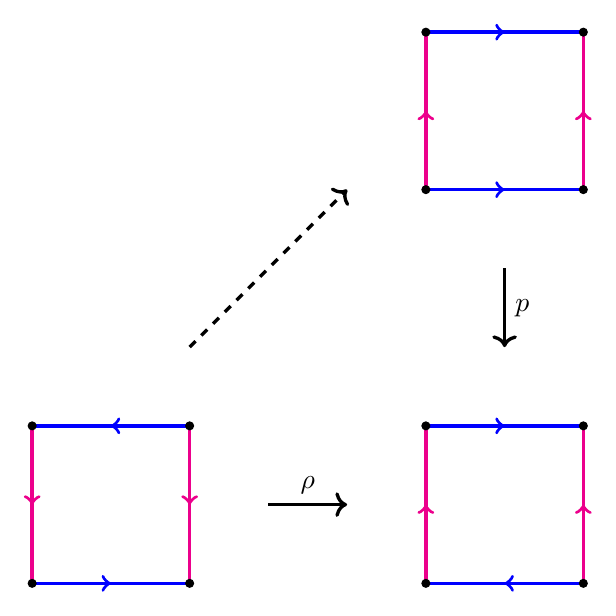
\begin{tikzpicture}[decoration={
					markings,
					mark=at position 0.5 with {\arrow{to}}
				}]
				\begin{scope}[shift={(0,5)}]
					\draw[magenta,very thick,postaction={decorate}] (0,0) -- (0,2);
					\draw[blue,very thick,postaction={decorate}] (0,2) -- (2,2);
					\draw[magenta,very thick,postaction={decorate}] (2,0) -- (2,2);
					\draw[blue,very thick,postaction={decorate}] (0,0) -- (2,0);
					% Vertices
					\filldraw (2,0) circle (0.05);
					\filldraw (2,2) circle (0.05);
					\filldraw (0,2) circle (0.05);
					\filldraw (0,0) circle (0.05);
				\end{scope}
				\begin{scope}[shift={(-5,0)}]
					\draw[magenta,very thick,postaction={decorate}] (0,2) -- (0,0);
					\draw[blue,very thick,postaction={decorate}] (2,2) -- (0,2);
					\draw[magenta,very thick,postaction={decorate}] (2,2) -- (2,0);
					\draw[blue,very thick,postaction={decorate}] (0,0) -- (2,0);
					% Vertices
					\filldraw (2,0) circle (0.05);
					\filldraw (2,2) circle (0.05);
					\filldraw (0,2) circle (0.05);
					\filldraw (0,0) circle (0.05);
				\end{scope}
				\begin{scope}
					\draw[magenta,very thick,postaction={decorate}] (0,0) -- (0,2);
					\draw[blue,very thick,postaction={decorate}] (0,2) -- (2,2);
					\draw[magenta,very thick,postaction={decorate}] (2,0) -- (2,2);
					\draw[blue,very thick,postaction={decorate}] (2,0) -- (0,0);
					% Vertices
					\filldraw (2,0) circle (0.05);
					\filldraw (2,2) circle (0.05);
					\filldraw (0,2) circle (0.05);
					\filldraw (0,0) circle (0.05);
				\end{scope}
				
				\draw[->,very thick] (1,4)--(1,3) node[midway, right] {$p$};
				\draw[->,very thick] (-2,1)--(-1,1) node[midway, above] {$\rho$};
				\draw[->,very thick,dashed] (-3,3)--(-1,5);
			\end{tikzpicture}\]
			Primero notemos que, por el teorema de Van Kampen, $\pi_1(K)\approx\langle a,b|abab^{-1}\rangle\approx\Z\rtimes\Z$, así que tenemos el siguiente diagrama de mapeos inducidos:
			\[\begin{tikzcd}
				&\Z\times \Z\arrow[d,"p_*"]\\
				\Z\rtimes\Z\arrow[r,swap,"\rho_*"]\arrow[ur]&\Z\rtimes\Z
			\end{tikzcd}\]
			Primero veamos cómo es la acción de $\rho_*$ en los generadores: $a\mapsto a^{-1}$ y $b\mapsto b^{-1}$, así que $\rho_*$ es un isomorfismo. Para saber cómo es la acción de $p_*$, vemos que $a\mapsto a$ y $b\mapsto b^{-1}$. Así, $p_*\pi_1(T)=\langle a,b^{-1}|ab^{-1}ab\rangle\approx\Z\rtimes\Z$. Concluimos que
			\[\rho_*\pi_1(K,k_0)\approx\Z\rtimes\Z\approx p_*\pi_1(T,t_0)\]
			Parece que el levantamiento invierte orientación ya que, al menos en términos de los generadores del grupo fundamental, manda $a\mapsto a^{-1}$.
		\end{proof}
		\item Si tomamos $S_g$ en lugar del toro, ¿qué es $S_g/\langle\sigma\rangle$? ¿Es cierto que $\chi(S_g)=2\chi(S_g/\langle\sigma\rangle)$. Recuerda que $\chi(S_g)=2-2g$ y $\chi(N_g)=2-g$.
	\end{enumerate}
\end{ejer}
\section{Cubrientes ramificados}
\begin{defn}
	Sean $E$ y $X$ dos variedades. Decimos que $p:E\to X$ es un cubriente ramificado si existe una subvariedad $B$ de codimensión 2 en $X$ tal que 
	\[p|_{E\backslash p^{-1}(B)}:E\backslash p^{-1}(B)\to X\backslash B\]
	es un espacio cubriente. Decimos que $B$ es el \textbf{conjunto de ramificación}, y $p^{-1}(B)$ es el \textbf{conjunto de puntos singulares} o \textbf{branch points}.
\end{defn}
\begin{ejem}
	$z\mapsto z^n$ actuando en el disco. El 0 es un punto de ramificación.
\end{ejem}
\begin{obs}
	Los puntos de ramificación localmente se ven como $z\mapsto z^n$, y éste número se llama \textbf{índice de ramificación}. Esto simplemente quiere decir que se trata de superficies de Riemann para las cuales existen cartas coordenadas complejas tal que la proyección se ve como $z\mapsto z^n$.
\end{obs}
\begin{teo}
	Si $G\curvearrowright S$ propiamente discontinuo, $p:S\to S/G$ es un cubriente ramificado regular.
\end{teo}
\begin{ejem}
	El toro rotando $\pi$ respecto al eje $x$. El cociente $T_2/\Z_2$ es una esfera con cuatro puntos de ramificación. Si en cambio tomamos $S_2$, el cociente es una esfera con 6 puntos de ramificación. En general, $S_g$ tiene $2g+2$ puntos de ramificación.
\end{ejem}
\begin{ejem}
	Girando un triple toro respecto a al eje $x$ y luego respecto al eje $y$, tenemos un cubriente de 4 hojas. Los puntos de ramificación, que son 6, son de índice 2. Notemos que 
	\[(\chi(S^2)-t)=\sum_{x\in B}|p^{-1}(x)|\]
	donde $B$ es el conjunto de puntos de ramificación.
\end{ejem}
\begin{teo}[Riemann-Hurwitz]
	Dado un cubriente ramificado $p:S\to S/G$ con $B\subseteq S/G$ el conjunto de puntos de ramificación. Entonces,
	\begin{align*}
		\chi(S)&=|G|\chi(S/G)-|G|\sum_{x\in B}\left(1-\frac{1}{n_x}\right)\\
		&=|G|(\chi(S/G)-|B|)+\sum_{x\in B}|p^{-1}(x)|
	\end{align*}
	donde $n_x=|G_x|$ es el tamaño del estabilizador de $x$.
\end{teo}
\begin{proof}
	Levantando una descomposición celular en el espacio base. Los vértices se pueden no levantar bien, y de ahí que restamos un término.
\end{proof}
\begin{obs}
	Para un cubriente $p:E\to X$ no ramificado de grado $n$,
	\[\chi(E)=n\chi(X)\]
	el siguiente teorema generaliza este resultado para cubrientes ramificados.
\end{obs}
\begin{teo}[Riemann-Hurwitz en general]
	Si $p:E\to X$ es un cubriente ramificado de $n$ hojas y $B\subseteq X$ es el conjunto de puntos de ramificación,
	\[\chi(E)=n(\chi(X)-|B|)+\sum_{x\in B}|p^{-1}(x)|\]
	Y si $p^{-1}(B)=\{e_1,\ldots,e_r\}\subset E$ y el índice de ramificación de $e_i$ es $d_i$, entonces
	\[\chi(E)=n\chi(X)-\sum_{i=1}^r(d_i-1)\]
\end{teo}
\begin{coro}[Desigualdad de Hurwitz]
	Dado un grupo finito $G$ que actúa en $S_g$ para $g\geq2$, entonces $|G|\leq84(g-1)$.
\end{coro}
\begin{obs}
	¿Será que existe algún grupo con $|G|=84(g-1)$ que actúa en $S_g$? Sí, se llaman grupos de Hurwitz.
\end{obs}
\begin{ejer}[\textcolor{magenta}{Tarea}]
	Encontrar un cubriente $\Sigma_g\to S^2$ con exactamente 3 puntos de ramificación. \textbf{Hint}: usar la involución hiperelíptica $\Sigma_g\to S^2$ con $2g+2$ puntos de ramificación y luego otro cubriente $S^2\to S^2$ que a "dos puntos los mande a tres".
\end{ejer}
\begin{proof}[Solución]
	Consideremos primero el caso del toro. La involución hiperéliptica actúa en el toro para generar una esfera con cuatro puntos de ramificación (un orbifold). Podemos luego hacer actuar en esta esfera una rotación de 120º cuyo eje pasa por dos de estos cuatro puntos e identifica los otros dos. La composición de los dos mapeos cocientes es una función del toro en la esfera con dos puntos que tienen una sola preimagen y un punto que tiene dos preimágenes.
	
	Para generalizar este razonamiento a la superficie de género $G$ simplemente debemos continuar haciendo rotaciones en la esfera para identificar puntos entre los $2g+2$ hasta tener solo tres. Al final, habrá dos puntos con una sola preimagen, y los demás tendrán preimágenes de distintas cardinalidades.
\end{proof}
\begin{ejem}
	Tomemos un cubriente ramificado de $\Sigma_g\to S^2$. Si $g\geq1$, entonces el número de puntos de ramificación es mayor o igual que 3.
\end{ejem}
\begin{ejer}[\textcolor{magenta}{Tarea}]
	Si $\Sigma_g\to S^2$ es un cubriente ramificado con 2 puntos de ramificación, entonces $g=0$, es decir, $S^2$.
\end{ejer}
\begin{proof}[Solución]
	Parece análogo al ejemplo anterior simplemente sustituyendo en la fórmula de Riemann-Hurwitz para llegar a una contradicción.
\end{proof}
Ahora estudiemos algo así como el regreso de Riemann-Hurwitz:

Supongamos que tenemos dos superficies $\Sigma_g$ y $\Sigma_h$ orientables. Para un número $d\in\N$ (que es como el número de hojas del cubriente) y particiones de este número (que son como los índices de ramificación de cada uno de los $k$ puntos de ramificación en sus $\ell_i$ preimágenes):
	\[d=(d_{11},\ldots,d_{1\ell_1}),\ldots,(d_{k1},\ldots,d_{k\ell_1})\]
donde $\sum_id_{ji}=d$.
Si además
	\[\chi(\Sigma_g)=d\chi(\Sigma_h)-\sum_{i=1}^k\left(\sum_{j=1}^{\ell_i}(d_{ij}-1)\right)\]
¿Bajo qué condiciones existe un cubriente $\Sigma_g\to\Sigma_h$ de $d$ hojas con esos puntos de ramificación y esos índices de ramificación?
\begin{itemize}
	\item Si $h\geq1$.
	\item $h=0$, a veces se puede. \textbf{Tarea:} ¿Qué condiciones en las particiones de la $d$ se necesitan en este caso?
\end{itemize}

\section{Mapping Class Group}
\begin{defn}
	Una superficie de género $g$ con $n$ ponchaduras y $b$ componentes frontera es una \textbf{superficie de tipo finito} y se denota por $S^n_{g,n}$.
\end{defn}
\begin{defn}
	Un \textbf{cross-cap} es quitarle un disco a una superficie y pegarle a una banda de Möbius a lo largo de la frontera de ese disco.
\end{defn}
\begin{ejer}
	¿Cuál es el género de un toro con un cross-cap? Es una esfera con tres cross-caps, género 3. Y un toro con tres cross-caps es una esfera con cinco cross-caps, y también es un bitoro con un cross-cap.
\end{ejer}
El chiste es que podemos representar cualquier superficie no orientable $N_g$ como una esfera con $g$ cross-caps.

\begin{defn}
	Consideremos el anillo $\A=S^1\times [0,1]$. La función
	\begin{align*}
		T:\A&\to\A\\
		(e^{2\pi i\theta},t)&\mapsto(e^{2\pi i\theta t},t)
	\end{align*}
	se llama \textbf{giro de Dehn}.
\end{defn}
\begin{obs}
	$T$ es la identidad en las tapas del anillo.
\end{obs}
\begin{defn}
	Para una superficie $\Sigma$, denotaremos por $\Homeo(\Sigma)$ a su \textbf{grupo de homeomorfismos}.
\end{defn}
\begin{obs}
	Es un grupo topológico con la topología compacto-abierto. Una base (o subbase?) de esta topología está dada por conjuntos de la forma $V(K,U)=\{f\in\Homeo(\Sigma):f(K)\subset U\}$ para $K$ compacto y $U$ abierto en $\Sigma$.
\end{obs}
\begin{defn}
		Una homotopía entre homeomorfismos tal que todos las funciones en medio son homeomorfismos se llama \textbf{isotopía}. Si $f$ y $g$ son isotópicas escribiremos $f\simeq g$.
\end{defn}
	Denotaremos por \[\Homeo_0(\Sigma)=\{f\in\Homeo(\Sigma):f\simeq\Id_\Sigma\}\]
	\[\Homeo(\Sigma;\partial\Sigma)=\{f\in\Homeo(\Sigma):f|_{\partial\Sigma}=\Id|_{\partial\Sigma}\}\]
	\[\Homeo^+(\Sigma;\partial\Sigma)=\{f\in\Homeo(\Sigma;\partial\Sigma):f\text{ preserva orientación}\}\]
	\begin{ejer}[\textcolor{magenta}{Tarea}]
		$\Homeo_0(\Sigma)\triangleleft\Homeo(\Sigma)$.
	\end{ejer}
	\begin{proof}
		Supongamos que $f\simeq\Id$ y $g\in\Homeo(\Sigma)$. Entonces hay una función continua $H:I\times\Sigma\to\Sigma$ tal que $H(0,p)=p$ y $H(1,p)=f(p)$ para $t\in I$ y $p\in\Sigma$. Luego,
		\begin{align*}
			\tilde{H}:I\times\Sigma&\to\Sigma\\
			(t,p)&\mapsto g\circ H\circ g^{-1}(p)
		\end{align*}
		Es tal que $H(0,p)=g(H(0,g^{-1}(p))=gg^{-1}(p)=p$ y $H(1,p)=g(f(g^{-1}(p))=gfg^{-1}(p)$, es decir $gfg^{-1}\simeq\Id$.
		\end{proof}
	\begin{defn}
		El \textbf{mapping class group} o \textbf{grupo modular} de una superficie $\Sigma$ es 
		\[\Mod(\Sigma;\partial\Sigma)=\Homeo(\Sigma;\partial\Sigma)\Big/\Homeo_0(\Sigma,\partial\Sigma)\]
	\end{defn}
	\begin{obs}\leavevmode
	\begin{itemize}
		\item 	El grupo modular es un grupo topológico con la topología cociente.
		\item También,
			\[\Mod(S_{g,n}^b):=\Homeo(\Sigma;\partial \Sigma)\Big/\text{isotopía}\]
		\item Una isotopía se puede pensar como un camino en el grupo de homeomorfismos, es decir, $\hat{H}:I\to\Homeo(\Sigma,\partial)$, así que cada clase de isotopía es una componente conexa de este grupo:
			\[\Mod(S_{g,n}^b):=\pi_0(\Homeo(\Sigma;\partial \Sigma))\]
		\item Una superficie de género $g$ con $n$ ponchaduras y $b$ componentes frontera es una \textbf{superficie de tipo finito} y se denota por $\Sigma^n_{g,n}$. Resultará que si $\Sigma$ es (\textcolor{magenta}{Tarea}) una superficie de tipo finito, entonces $\Mod(\Sigma;\partial\Sigma)$ es un grupo discreto.
	\end{itemize}
	\end{obs}
	\begin{ejem}[Grupo modular del disco]
		$\Mod(\D^2,\partial\D^2)\approx\{1\}$.
	\end{ejem}
	\begin{proof}
		Cualquier función en el disco que fija la frontera es isotópica a la identidad. Definamos la isotopía geométricamente. Buscamos una función
		\begin{align*}
			H:\D^2\times I&\to\D^2\\
			(x,t)&\mapsto
			\begin{aligned}
				\begin{cases}
				(1-t)f(\frac{x}{1-t})&\qquad0\leq|x|\leq1-t\\
				x&\qquad1-t\leq|x|\leq1
			\end{cases}
			\end{aligned}
		\end{align*}
		es tal que $H(-,0)=f$ y $H(-,1)=\Id_{\D^2}$.
		
		La idea geométrica es, en el cilindro relleno $\D^2\times I$, colapsar el disco que es una de las tapas a un punto en la tapa opuesta. De hecho, en cada altura tenemos un círculo está dado por $|x|=1-t$. \textbf{Faltaría} ver que tenemos un homeomorfismo en cada $t$.
	\end{proof}
	\begin{ejem}[Grupo modular del anillo]
		$\Mod(\A;\partial\A)\approx\Z$
	\end{ejem}
	\begin{proof}
		Podemos pensar $\A$ como una superficie de género 0 ($S^2$) con dos componentes frontera y ninguna ponchadura.
		
		El cubriente universal de $\A$ es $I\times\R$.
		
		Tomemos $[f]\in\Mod(\A,\partial\A)$, y $\alpha$ la curva que une en línea recta $(0,0)$ y $(0,1)$. Luego, $f(\alpha)$ es una curva que puede darle ciertas vueltas al cilindro, pero termina en el mismo punto. Un levantamiento $\widetilde{f(\alpha)}$ está únicamente determinado por su imagen en un sólo punto. \textcolor{orange}{Creo que} esto obliga al levantamiento a ser una traslación en la banda $\R\times I$ de tantas unidades como el número de vueltas que le da al cilindro la curva $f(\alpha)$.
		\[\begin{tikzcd}
			&\R\times I\arrow[d,"p"]\\
			\A\arrow[ur,"\widetilde{f(\alpha)}"]\arrow[r,"f",swap]&\A
		\end{tikzcd}\]
		Esta transformación en el cubriente está bien definida y no depende del representante. Así, hemos construido una correspondencia $[f]\mapsto k_f$ donde $k_f$ es una traslación. Demostrar que esta función es suprayectiva no es trivial, pero es cierto.
	\end{proof}
	\begin{ejem}[Grupo modular de la banda de Möbius]
		$\Mod(\M;\partial\M)=\{\Id\}$.
	\end{ejem}
		\begin{ejem}[Grupo modular de la esfera, \textcolor{magenta}{Tarea}]
		$\Mod(S^2)=\{\Id\}$.
	\end{ejem}
	\begin{proof}
		Hint: usar que cualquier homeomorfismo se puede homotopear a un homeomorfismo que tiene un punto fijo.
	\end{proof}
	\begin{ejem}[Grupo modular del toro]
		$\Mod(T^2)\approx\SL_2(\Z)$
	\end{ejem}
	\begin{proof}
		Mediante un mapeo
		\begin{align*}
			\Phi:\Mod(T^2)&\to\SL_2(\Z)\\
			\begin{aligned}
				[f]\mapsto\\\\
			\end{aligned}&
			 \begin{aligned}
				f_*:H_1(T^2)&\to H_1(T^2)\\
				\langle a\rangle\times\langle b\rangle&\to\langle a\rangle\times\langle b\rangle
			\end{aligned}
		\end{align*}
		que resulta ser suprayectivo e inyectivo. En algún momento usamos el cubriente del toro, el plano.
	\end{proof}
	\begin{ejem}[Grupo modular del plano proyectivo]
		$\Mod(\R P^2)\approx\{\Id\}$
	\end{ejem}
	\begin{proof}
		Cortando el hemisferio superior de la esfera a lo largo de un paralelo.
	\end{proof}
	
\section{Teorema de Birman-Hilden}
Primero observamos que podemos tomar clases de isotopía y clases de homotopía indistintamente, y también, que se pueden tomar difeomorfismos en vez de homeomorfismos.
\begin{obs}\leavevmode
	\begin{itemize}
		\item Let $\Sigma$ be any compact surface, and let $f$ and $g$ be homotopic homeomorphisms of $\Sigma$. Then $f$ and $g$ are isotopic unless they are one of the two examples described above (on $\Sigma = \D^2$ and $\Sigma=\A$). In particular, if $f$ and $g$ are orientation-preserving then they are isotopic.
		\item Let $\Sigma$ be a compact surface. Then every homeomorphism of $\Sigma$ is isotopic to a diffeomorphism of $\Sigma$.
	\end{itemize}
\end{obs}
Tomemos un cubriente ramificado $p:S\to X$ con $S$ y $X$ superficies orientables. Sea $B\subset X$ el conjunto de puntos de ramificación de $p$. Trabajaremos con homeomorfismos que fijen $B$. Esto se puede expresar de esta forma:
\[\Mod(X\backslash B)\approx\Mod_{k}X,\qquad k=|B|\]
	
Dado un homeomorfismo de $S$, ¿cuándo podemos definir un homeomorfismo de $X$?
\[\begin{tikzcd}
	S\arrow[r,"\tilde{f}"]\arrow[d,"p",swap]&S\arrow[d,"p"]\\
	X\arrow[dashed,r,"f"]&X
\end{tikzcd}\]
Basta pedir que $f$ preserve las fibras, es decir, que $\tilde{f}(p^{-1}(x))=p^{-1}(y)$ para algún $y\in X$. O bien, $f(\tilde{x})=f(\tilde{x}')$ para $\tilde{x}$ y $\tilde{x}'$ en la misma fibra de algún punto en $X$.

Denotemos
\[\mathcal{S}\Homeo(S)=\{\tilde{f}\in\Homeo(S):\tilde{f}\text{ preserva fibras de }p\}\]
\[\mathcal{L}\Homeo(X)=\{f\in\Homeo(X\backslash B):f\text{ se levanta bajo }p\}\]
\begin{obs}
	Para un cubriente ramificado $p:S\to X$, existe un \textbf{homomorfismo natural}
	\begin{align*}
		\Phi:\mathcal{S}\Homeo&\to\mathcal{L}\Homeo(X)\\
		\tilde{f}&\mapsto f
	\end{align*}
	Pero al contrario no siempre es cierto, pues para cada función levantable hay muchos posibles levantamientos.
\end{obs}

	La proyección natural
	\begin{align*}
		\pi:\Homeo(S)&\to\Mod(S)\\
		f&\mapsto [f]
	\end{align*}
	nos permite definir
	\begin{align*}
		\SMod(S):&=\pi(\mathcal{S}\Homeo(S))\\
		&=\{[\tilde{f}]\in\Mod(S):\exists\tilde{f}'\in\mathcal{S}\Homeo(S)\text{ con }\tilde{f}\simeq\tilde{f}'\}
	\end{align*}
	Es decir, son las clases de isotopía en el grupo modular que contienen al menos un elemento que preserva fibras. El \textbf{grupo modular simétrico} de $S$ es precisamente $\SMod(S)<\Mod(S)$.
	
	Análogamente, tenemos la proyección
\begin{align*}
	\pi:\Homeo(X\backslash B)&\to\Mod_k(X)\\
	f&\mapsto [f]
\end{align*}
nos permite definir
\begin{align*}
	\LMod(X):&=\pi(\mathcal{L}\Homeo(X))\\
	&=\{[f]\in\Mod_k(X):\exists f'\in\mathcal{L}\Homeo(X)\text{ con }f\simeq f'\}
\end{align*}
que llamaremos el \textbf{grupo modular levantable} de $S$.

En qué casos podemos extender una función $\phi$ como a continuación?
\[\begin{tikzcd}
	\SHomeo(S)\arrow[r,"\phi"]\arrow[d,"\pi",swap]&\LHomeo(X)\arrow[d,"\pi"]\\
	\SMod(S)\arrow[dashed,r,"\Phi"]&\LMod(X)\}\\
	\left[f\right]\arrow[maps to]{r}&\left[\phi(f)\right]
\end{tikzcd}\]
Primero debemos ver que dado $[\tilde{f}]\in\SMod(S)$, si $\tilde{g},\tilde{g}'\in\SHomeo(S)$ están en la clase de $\tilde{f}$, entonces $\Phi(\tilde{g})\simeq\Phi(\tilde{g}')$. Para esto, basta ver que la proyección cubriente preserva homotopías.

Específicamente, para $H:S\times I\to S$ con $H(-,0)=\tilde{g}$ y $H(-,1))=\tilde{g}'$ hay un $\bar{H}:X\times I\to X$ con $\bar{H}(-,0)=\phi(\tilde{g})$ y $\bar{H}(-,1)=\phi(\tilde{g}')$.

Uno puede garantizar esto si $h_t:=H(-,t)\in\SHomeo(S)$ para toda $t$. De hecho, es suficiente mostrar que existe un map isotópico a la identidad que preserve fibras, pues
\begin{align*}
	\tilde{g}\simeq\tilde{g}'&\implies\phi(\tilde{g})\simeq\phi(\tilde{g}')\\
	\iff\tilde{g}\circ\tilde{g}^{-1}\simeq\Id_S&\iff\phi(\tilde{g}\circ\tilde{g}^{-1}\simeq\Id_X)\iff f\simeq\Id_S
\end{align*}
con $f\in\SHomeo(S)$ mediante una homotopía $H:S\times I\to S$ tal que $H(-,t)\in\SHomeo(S)\iff\phi(f)\simeq\Id_X$.

\begin{defn}
	Sea $p:S\to X$ un cubriente ramificado. Decimos que $p$ satisface la \textbf{propiedad de Birman-Hilden} si para cada $g\in\SHomeo(S)\cap\Homeo_0(S)$ existe una isotopía $H:S\times I\to S$ tal que $h_t:=H(-,t)\in\SHomeo(S)$. Es decir, existe una isotopía con la identidad de $S$ que preserva fibras del cubriente.
\end{defn}
\begin{obs}
	Un cubriente $p$ satisface la propiedad de Birman-Hilden si y sólo si la función natural $\Phi:\SMod(S)\to\LMod(X)$ está bien definida.
\end{obs}
\begin{ejem}
	Tomemos $S=T^2$ como cubriente de $S^2$ mediante la involución hiperelíptica, que tiene cuatro puntos de ramificación. Consideremos también $\tilde{f}$ la rotación en el eje $Z$ por $\pi$, que es homotópica a la identidad. Además, $\tilde{f}$ preserva fibras, ¿por qué? Este cubriente no satisface la condición de Birman-Hilden.
\end{ejem}
\begin{teo}[Birman-Hilden]
	Sea $p:S\to X$ un cubriente ramificado y regular con número finito de hojas, con $\chi(S)<0$. Si $p$ no es ramificado o \textbf{soluble} ($p_*(\pi_1(S\backslash B))\triangleleft\pi_1(X\backslash B)$ es soluble), entonces $p$ tiene la propiedad de Birman-Hilden.
\end{teo}
Agregamos este comentario rápidamente:
\begin{defn}[\cite{Rotman}, p.464]
	Una \textbf{\textit{serie normal}} de un grupo $G$ es una sucesión de grupos 
	\[G=G_0\geq G_1\geq G_2\geq\ldots\geq G_t=\{1\}\]
	con cada $G_{i+1}$ un subgrupo normal de $G_i$; los \textbf{\textit{grupos factores}} de esta serie son los cocientes
	\[G_0/G_1,\quad G_1/G_2,\quad\ldots\quad G_{t-1}/G_t\]
	Un grupo finito $G$ es \textbf{\textit{soluble}} si $G=\{1\}$ o $G$ tiene una serie normal cuyos grupos factores son de orden finito.
\end{defn}

Antes de demostrarlo, probaremos que:
\begin{teo}
	Sea $p:S\to X$ un cubriente ramificado regular con un número finito de hojas $g$ y una cantidad finita de puntos de ramificación. Supongamos que cada transformación cubriente deja fijo el conjunto de puntos de ramificación y que $S$ es hiperbólica.  Entonces $p$ satisface la condición de Birman-Hilden.
\end{teo}

Comenzaremos con
\paragraph{Paso 1} Sea $B\subset X$ el conjunto de puntos de ramificación. Si $f\in\SHomeo(S)\cap\Homeo_0(S)$, entonces $f(\tilde{x})=\tilde{x}$ para cualquier $\tilde{x}\in p^{-1}(B)$.

\begin{defn}
	Una \textbf{superficie de Riemann} $S$ es una superficie para la cual los cambios de coordenadas son analíticos en el sentido complejo, es decir, $\partial_zf=0=\frac{1}{2}(\partial_xf-i\partial_yf)$.
\end{defn}
\begin{obs}
	Si $p:S\to X$ es un cubriente ramificado, podemos pensar que en las estructuras de superficie de Riemann, de manera que $p:(S,Y)\to(X,Z)$ es analítico en el sentido complejo. En este contexto, las transformaciones de cubierta son analíticas.
\end{obs}
\begin{ejer}[\textcolor{magenta}{Tarea}]\leavevmode
	\begin{itemize}
		\item Si $\chi(S)<0$, entonces $Z(\pi_1(S))$ es trivial. \textcolor{magenta}{Dani}
	\begin{proof}\textit{Otra idea, más geométrica:}
			
			Primero observemos que una superficie sin frontera $S$ con $\chi(S)<0$ \href{https://mathoverflow.net/questions/14548/finding-constant-curvature-metrics-on-surfaces-without-full-power-of-uniformiza}{admite una métrica Riemanniana de curvatura constante} negativa. Para verlo, basta mostrar que cualquier superficie de género $g$ se puede ver topológicamente como un polígono de $4g$ lados identificados adecuadamente.
			
			En el caso del toro, podemos usar un cuadrado e identificar sus lados como es usual. La observación clave es que el plano euclideano se puede teselar con copias de este cuadrado, y el grupo de traslaciones que envía un cuadrado en otro $\Z\times\Z$ es un grupo de isometrías del plano.
			
			El plano hipérbolico tiene la increíble propiedad de que puede ser teselado por polígonos regulares de cualquier número de lados, en particular con un $4g$-ágono cuyos lados se identifquen para construir nuestra superficie. El grupo de traslaciones hiperbólicas que lleva copias del polígono en otras copias es un subgrupo de isometrías del plano hiperbólico. De hecho, se puede escoger un grupo $\Gamma$ con esa propiedad tal que el cociente $\Hy^2/\Gamma$ sea homeomorfo a nuestra superficie.
			
			A partir de aquí el argumento es como en la prueba anterior.
			
			Estas ideas también están el Lee, Introduction to Riemannian Manifolds.
		\end{proof}
		\item Si $f\in\Homeo(S)$ tal que $f_*:\pi_1(S)\to\pi_q(S)$ es la identidad, entonces $f\simeq\Id_S$.
		\item Si el mapeo además es analítico, entonces de hecho $f$ es la identidad, es decir $f\in\Homeo(S)\cap\Homeo_0(S)$ es analítico, $f=\Id_S$.
	\end{itemize}
\end{ejer}
\begin{lema}
	Sea $f\in\Homeo(S)\backslash\{\Id\}$ tal que $f$ fija un punto $\tilde{x}\in S$. Consideremos \[f_*:\pi_1(S,\tilde{x})\to\pi_1(S,\tilde{x})\]
	Entonces,
	\[f_*([\gamma])=[\gamma]\implies[\gamma]=1\]
\end{lema}
\begin{proof}
	Sea $[\gamma]\in\pi_1(S,\tilde{x})\backslash\{1\}$ tal que $f_*([\gamma])=[\gamma]$. Tenemos que \[f(\gamma)\simeq\gamma\rel\tilde{x}\]
	También tenemos el cubriente universal $q:\Hy^2\to S$, y podemos levantar $f$:
	\[\begin{tikzcd}
		(\Hy^2,\xi)\arrow[r,"\tilde{f}"]\arrow[swap,d,"q"]&(\Hy^2,\xi)\arrow[d,"q"]\\
		(S,\tilde{x})\arrow[r,"f"]&(S,\tilde{x})
	\end{tikzcd}\]
	Como $f$ es analítico, $\tilde{f}\in\Isom^+(\Hy^2)$. Tomando $\gamma:I\to S$ con $\gamma(0)=\gamma(1)=\tilde{x}$, tenemos:
	\[\begin{tikzcd}
		&(\Hy^2,\xi)\arrow[d,"q"]\\
		(I,0)\arrow[r,"\gamma"]\arrow[ur,dashed,"\tilde{\gamma}"]&(S,\tilde{x})
	\end{tikzcd}\]
	Es decir, tenemos $\tilde{\gamma}:I\to S$ tal que $\tilde{\gamma}(0)=\xi$. Llamemos $\xi'=\tilde{\gamma}(1)\neq\xi$.
	
	Por otro lado, $f(\gamma)\simeq\gamma\rel\tilde{x}$, entonces $\widetilde{f(\gamma)}(1)=\tilde{\gamma}(1)=\xi'$. Pero $\widetilde{f(\gamma)}=\tilde{f}\tilde{\gamma}$ y así
	\[\tilde{f}\xi'\text{*\textbf{falta}*}\]
\end{proof}

\begin{lema}
	Sea $\tilde{g}\in\SHomeo(S)\cap\Homeo_0(S)$. Entonces $\tilde{g}$ conmuta con las transformaciones de cubierta.
\end{lema}
\begin{proof}
	Sea $\tau\Deck(p)$, de manera que
	\[\begin{tikzcd}
		S\arrow[rr,"\tau"]\arrow[dr,"p",swap]&&\textcolor{blue}{S}\arrow[dl,"p"]\arrow[r,"\tilde{g}^{-1}",blue]&S\arrow[r,"\tau"]\arrow[d,"p",blue]&S\arrow[dl,"p"]\arrow[r]&S\arrow[d,"p",blue]\\
		&X\arrow[rr,blue,swap,"g^{-1}"]&&\textcolor{blue}{X}\arrow[rr,"g",blue]&&\textcolor{blue}{X}
	\end{tikzcd}\]
	Definiendo
	\[r:=\tilde{g}\circ\tau\circ\tilde{g}^{-1}\in\Deck(p)\]
	tenemos que:
	\begin{enumerate}
		\item $r\simeq\Id_S$.
		\item $r$ fija los puntos de ramificación del cubriente $p:S\to X$.
	\end{enumerate}
	Dado un punto de ramificación $\tilde{x}_1\in S$, tenemos que 
	\[\textcolor{magenta}{r_*:\pi_q(S,\tilde{x}_1)\to\pi_1(S,\tilde{x}_1)}\]
	es un automorfismo interno de $\pi_1(S,\tilde{x}_1)$, entonces existe $[\beta]\in\pi_1(S,\tilde{x}_1)$ \textcolor{magenta}{(faltó ver que $[\beta]\neq1$)} tal que $r_*([\gamma])=[\beta\cdot\gamma\cdot\beta^{-1}]$.
	
	Ahora si $r\neq\Id_S$, como $r$ es analítico y fija un punto por el lema anterior,
	\[r_*([\beta])=[\beta\cdot\beta\cdot^{-1}]=[\beta]\implies[\beta]=1\]
	Entonces $r_*=\Id_S$, y de hecho, por tratarse de una superficie hiperbólica, $r=\Id$. Para concluir, simplemente notamos que $\tilde{g}\tau\tilde{g}^{-1}\tau^{-1}=\Id_S\implies \tilde{g}\tau=\tau\tilde{g}$ para cualquier $\tilde{\tau}\in\Deck(p)$.
\end{proof}
\begin{lema}
	Si $\tilde{g}\in\SHomeo(S)\cap\Homeo_0(S)$ con una homotopía $G:S\times I\to S$ tal que $G(\tilde{x},0)=\tilde{x}$ y $G(\tilde{x},1)=\tilde{g}(\tilde{x})$.
	\begin{enumerate}
		\item $\tilde{g}(\tilde{x}_i)=\tilde{x}_i$ para $i=,1,\ldots,n$. $pi^{-1}(B)=\{\tilde{x}_1,\ldots,\tilde{x}_n\}$.
		\item El lazo $\beta_i=G(\tilde{x},-)$ es homotópico al lazo constante en $\pi_1(S,\tilde{x}_i)$.
	\end{enumerate}
\end{lema}
\begin{proof}\leavevmode
	\begin{enumerate}
		\item Por contradicción, supongamos que $\tilde{g}(\tilde{x}_i)\neq\tilde{x}_i$, de manera que, como estamos suponiendo que las transformaciones cubrientes fijan el conjunto de puntos de ramificación, $\tilde{g}(\tilde{x}_i)=\tilde{x}_j$ con $i\neq j$.
		
		Tomemos un lazo $\gamma$ basado en $\tilde{x}_i$ y $\tau\in\Deck(p)\backslash\{\Id\}$. Por el lema anteior, $\gamma$ conmuta con $\tau$.
		\begin{equation}\label{ec:1}
			\tilde{g}\tau=\tau\tilde{g}
		\end{equation}
		Definamos $\beta(t)=G(\tilde{x},t)$. Entonces,
		\[\gamma\simeq\beta\cdot\tilde{g}(\gamma)\cdot\beta^{-1}\]
		pues $\tilde{g}\simeq\Id\rel\tilde{x}_i$.
		
		Aplicando $\tau$ a lo anterior, (ya que $\tau(\tilde{x}_i)=\tilde{x}_i)$,
		\begin{equation}\label{ec:2}
			\tau(\gamma)\simeq\tau(\beta)\cdot\tau\tilde{g}(\gamma)\cdot\tau(\beta^{-1})
		\end{equation}
		Como $\gamma$ es arbitrario, pongamos $\tau(\gamma)$ y
		\begin{equation}\label{ec:3}
			\tau)\gamma\simeq\beta\cdot\tilde{g}(\tau(\gamma))\cdot\beta^{-1}
		\end{equation}
		Por \eqref{ec:1}, $\tau(\gamma)\simeq\beta\cdot\tau\tilde{g}(\gamma)\cdot\beta^{-1}$, y por \eqref{ec:2},
		\begin{align*}
			\tau(\beta)\cdot\tau\tilde{g}(\gamma)\cdot\tau(\beta^{-1})=\beta\cdot\tau\tilde{g}(\gamma)\cdot\beta^{-1}\\
			\implies (\beta^{-1}\cdot\tau(\beta))\cdot\tau\tilde{g}(\tau)\cdot(\tau(\beta^{-1})\cdot\beta)\simeq\tau\tilde{g}(\gamma)
		\end{align*}
		\textcolor{cyan}{Como $\gamma$ fue arbitrario, podemos reemplazar $\gamma=t^{-1}g^{-1}(\gamma)$.}
		
		Para probar que el lazo $\beta^{-1}\cdot\tau(\beta)$ conmuta con todos los elementos de $\pi_1(S,\tilde{x}_j)$. Luego
		\[[\beta^{-1}\cdot\tau(\beta)\in Z(\pi(S,\tilde{x}_j))\approx\{\Id\}]\]
		Entonces,
		\[\beta^{-1}\cdot\tau(\beta)\simeq c_{\tilde{x}_j}\]
		Luego entonces,
		\[\tau(\beta)\simeq\beta\rel\tilde{x}_i,\tilde{x}_j\]
		\begin{af}
			$\tau=\Id_S$.
		\end{af}
		\[\begin{tikzcd}
			(\Hy^2,\xi_i)\arrow[r,"\tilde{\tau}"]\arrow[d,"q",swap]&(\Hy^2,\xi_i)\arrow[d,"q"]\\
			(S,\tilde{x}_i)\arrow[r,swap,"\tau"]&(S,\tilde{x}_i)
		\end{tikzcd}\]
		Consideremos $\tilde{\beta}=\xi_i$, de forma que $\tilde{\beta}(1)=\xi_j\in q^{-1}(\tilde{x}_j)$.
		\[\widetilde{\tau(\beta)}=\tilde{\tau}(\tilde{\beta}(1))=\tilde{\tau}(\xi_j)=\tilde{\tau}(\xi_j)=\xi_j\]
		Entonces, $\tilde{\tau}$ fija dos puntos, así que $\tau=\Id_{\Hy^2}$, y entonces $\tau=\Id_S$.
		
		Esta afirmación nos lleva a una contradicción, pues supusimos que $\tau\in\Deck\backslash\{\Id\}$.
		\item \textcolor{red}{Tarea: pruebe que $\pi_1(S)$ con $\chi(S)<0$ es libre de torsión.}
		\item \textcolor{red}{Si}
		\[\begin{tikzcd}
			S\arrow[d,"p"]\arrow[r,"\pi_1"]&S/H\arrow[dl,"\pi_2"]\\
			S/G
		\end{tikzcd}\]
	\textcolor{red}{Con $H\triangleleft G$. Si $\pi_1$ y $\pi_2$ (las proyecciones cociente) satisfacen Birman-Hilden, entonces $p:S\to S/G$ también.}
	\end{enumerate}
\end{proof}
\begin{teo}[Dehn-Nielsen-Baer]
	\[\Mod^\pm(S)\approx\operatorname{Aut}\pi_1(S,x_0)\Big/\img(\pi_1(S,x_0))\]
\end{teo}
\begin{proof}
		\[\begin{tikzcd}[row sep=tiny]
		\pi_1(S,x_0)\arrow[r,"f_*"]&\pi_1(S,f(x_0))\arrow[r,"c_\beta"]&\pi_q(S,x_0)\\
		\left[\gamma\right]\arrow[r,maps to]&\left[f(\gamma)\right]\arrow[r,maps to]&\left[\beta\circ f(\gamma)\circ \beta^{-1}\right]
	\end{tikzcd}\]
\end{proof}

\begin{teo}[1]
	Sea $p:S\to X$ un cubriente regular, ya sea ramificado o no ramificado con a lo más un número finito de puntos de ramificación. Supongamos que el grupo de transformaciones de cubierta $G=\Deck(p=)$ es soluble y finito. Si $\tilde{g}\in\SHomeo(S)\cap\Homeo_0(S)$, entonces el homeomorfismo $g:X\to X$ tal que
	\[\begin{tikzcd}
		S\arrow[r,"\tilde{g}"]\arrow[swap,d,"p"]&S\arrow[d,"p"]\\
		X\arrow[r,"g"]&X
	\end{tikzcd}\]
	es isotópico a la identidad en $X$, es decir, $g\in\Homeo_0(X)$.
\end{teo}
\begin{lema}
	Si $p:S\to X$ es un cubriente con las propiedades del teorema 1 y es tal que $|G|$ es primo, entonces para cualquier $\tau\in\Deck(p)$ se tiene que $\tau(\tilde{x})=\tilde{x}$ para cualquier $\tilde{x}\in p^{-1}(B)$ donde $B\subseteq X$ es el conjunto de puntos de ramificación.
\end{lema}

\iffalse
\begin{defn}
	Las transformaciones \textbf{levantables}, son las que satisfacen la propiedad del levantamiento y de denotan por $\mathcal{L}\Mod(S)$.
\end{defn}
\begin{obs}
	Para un cubriente $p: E\to X$ y una función $\tilde{f}: E\to E$ que preserva fibras, podemos definir una función $f:X\to X$.
\end{obs}
\begin{defn}
	Las transformaciones \textbf{simétricas}, son automorfismos del cubriente que preservan fibras y de denotan por $\mathcal{S}\Mod(S)$.
\end{defn}
¿Cómo podemos relacionar $\LMod(S)$ y $\SMod(S)$? Necesitamos una isotopía entre dos transformaciones simétricas por transformaciones simétricas.
\begin{pregunta}\leavevmode
	\begin{itemize}
		\item ¿Cómo debe ser el cubriente para que existan funciones
		\[\SMod( E)\to\LMod(X)\qquad\LMod(X)\to\SMod( E)\text{?}\]
		\item ¿Bajo qué condiciones se dan las igualdades
		\[\LMod(X)=\Mod(X)\qquad\SMod( E)=\Mod( E)?\]
		\item Para el grupo de trenzas $B_k$,
	\end{itemize}
\end{pregunta}\fi
\end{document}